\section{2021年校赛-多频点合成模拟信号数据传输系统}
\subsection{问题分析}
本题的软件任务分为接收端和发送端两部分,需要使用两块STM32F1单片机完成。发送端接受上位机的比特流,
编码为多频点信号并输出;接收端采样模拟信号并恢复其中编码的信息,传回上位机。

以下对两部分工作进行分析,统一起见,分别简称为RX和TX(注意这是相对于上位机而言的,
和题目中称呼刚好相反)

\subsection{RX-多频信号合成端}
\subsubsection{方案总览}
在一个典型工作流中,RX端需要完成的任务如下:

\begin{enumerate}
  \item \label{itm:rx-1} 接收上位机(电脑)通过UART传来的字节流
  \item \label{itm:rx-2} 将字节流按4比特为单位进行拆分,合成最多4个频点的模拟信号
  \item \label{itm:rx-3} 将多频点信号通过DAC进行输出
\end{enumerate}

步骤\Cref{itm:rx-1}和步骤\Cref{itm:rx-2}实际上是异步的前后台关系,因为上位机数据传输的时机、
数据量都不确定,因此需要非阻塞接收,放入待处理队列中(后台);在主循环(前台)中,
则从队列中取出数据进行合成,因此整个处理过程宜把单个字节作为基本单位。

用于表征比特状态的4个单频信号,分别选择\SI{4}{kHz}、\SI{8}{kHz}、\SI{12}{kHz}、
\SI{19}{kHz},这保证了频点间隔足够大,方便TX端进行区分。另外,由于中间模拟传输过程是异步的,
因此在空闲时也需要输出一个这四个频率之外的导频信号,供TX端检测有效信号的起始与结束。
在此选择了\SI{30}{kHz}的正弦波作为导频信号,以尽量减少空闲检测时间。

信号合成选用\textbf{直接数字频率合成}(DDS)技术,因为这样最通用,
可以合成出一定范围内的所有频率信号。其他可行的方案包括\textbf{动态计算正弦值}、
\textbf{为四个频率分别生成查找表}等,前者最节省空间,但时延过高因此不予考虑;
后者看似浪费大量空间,实际上对于本问题来说也是较优的方案,因为我们选择的频点具有简单的倍数关系,
在查找表的大小上,只需要保证频率最低的频点有完整的一个周期,另外几个更高的频点也自然具有完整的
多个周期,因此在截断问题上,不需要很多的空间就可以保证较小的频谱泄漏;
而DDS方案由于需要保证合成频率精度,需要的正弦查找表大小可能与该方案不相上下。
但考虑到DDS方案可以方便修改频率而无须重新生成查找表的优点,因此仍然采用DDS方案。

DAC输出采用DMA搬运数据+定时器Update事件触发转换的方式。由于我们比较关心信号的连续性和持续时间,
因此将DMA设置为连续(Circular)模式,在固定时延后手动停止DMA传输即可。
定时器触发频率和DDS的采样频率保持一致,通过正确设置基本定时器的预分频寄存器和自动重装载寄存器
可以达到这点,具体分析可参考前文\Cref{sec:tim}(微秒延时)部分,
其中基本定时器的配置在F1和H7上都是类似的。

\subsubsection{数据接收}
从上位机电脑发来的数据需要实时接收,在UART中断回调函数中放入待处理队列。队列可简单定义成一个singleton:

\begin{cbox}{queue.c}
static struct
{
  qsize_t head;
  qsize_t tail;
  qdata_t data[QUEUE_MAX_SIZE];
} g_queue;
\end{cbox}

由于本题中,电脑端下行比特数不超过160,因此队列最大容量\cinl{QUEUE_MAX_SIZE}设置为20。

队列的实现对外提供基本操作接口,供上层应用调用。其中两个比较重要的接口定义如下:

\begin{cbox}{queue.h}
/**
 * UART接收的数据,通过此函数放入数据队列
 */
void queue_push(qdata_t data);

/**
 * 从队列中取出一个数据
 *
 * @return  -- 1: 队列非空,数据有效
 *          -- 0: 队列为空,数据无效
 */
qsize_t queue_pop(qdata_t *data);
\end{cbox}

在前台主循环中,检测队列中是否有待处理数据,如是则取出进行处理。由于需要确认数据的有效性,
因此为数据格式增加一个相应的标识:

\begin{cbox}{receiver.h}
typedef struct
{
  uint8_t data;
  bool is_valid;  /* 用于区分有效的0和无效的0 */
} result_t;
\end{cbox}

\subsubsection{频率合成}
根据DDS的原理,有

\begin{equation}
  f_\textrm{out} = \frac{M\times f_\textrm{s}}{2^n}
\end{equation}

其中,$M$是频率调谐字(Frequency Tuning Word),在每次迭代中作为相位累加器的输入;
$f_\textrm{s}$是信号采样频率,在这里我们不妨设为\SI{300}{kHz},
既保证了十倍于最大所需频率(\oldSI{30}{kHz}),也兼顾了硬件性能;$n$是相位累加器的宽度,
也即一个圆周被分成的份数($2^n$)。

我们想要将合成频率误差控制在$2\%$以内,也即对于频率最低的信号\SI{4}{kHz},满足

\begin{equation}
  \frac{f_\textrm{s}}{2^n} \le \oldSI{4}{kHz}\times 2\%\times 2
\end{equation}

代入得

\begin{equation}
  n \ge \log_2{1875.0}=10.87\approx 11
\end{equation}

故正弦查找表的深度可以确定为11位(即圆周2048等分)。进一步,可以只使用前四分之一的采样,
其余部分的采样值可通过判断相位取值区间简单地映射到前四分之一,于是我们只需要512个采样点。
使用MATLAB生成正弦查找表的代码参见文件\cinl{sinlut_gen.m}.

\subsubsection{信号输出}
在上一阶段中生成的取样信号,需要通过DAC输出。传输的基本单位是一个字节,拆分成高低4个比特,
以小端格式分两次传输,即先低4比特再高4比特。一个字节输出的典型时序如下(两端都是足够长的导频信号):

\begin{table}[H]
\center
\begin{tabular}{cc|c|c|c|c}
    \cline{2-6}
    \multirow{1}{*}{信号内容} & ... & 多频点信号(低4比特)& 导频信号 & 多频点信号(高4比特)& ...\\
    \cline{2-6}
    \multirow{1}{*}{持续时间} & \multicolumn{1}{c}{} &
    \multicolumn{1}{c}{\cinl{ELAP_SIGNAL}} & \multicolumn{1}{c}{\cinl{ELAP_FREQ_D}} &
    \multicolumn{1}{c}{\cinl{ELAP_SIGNAL}} & \multicolumn{1}{c}{}
\end{tabular}
\captionof{table}{信号输出时序}
\end{table}

其中两个持续时间\cinl{ELAP_SIGNAL}和\cinl{ELAP_FREQ_D}待定,需要根据TX端的ADC采样、
处理时间来进一步确定。实际上该时序还有进一步的优化空间,只要我们能确定TX端的最大处理延时,
便可以在适当调整有效信号持续时间的前提下,放心地去掉高低4比特之间的导频信号。
由于TX端采样、处理仍是以4比特为单位,去掉这段导频信号后可能会带来同步失败的问题,但只要有了确定时延,
便可以保证第二次采样区间落在高4比特信号的范围内。本质是将同步单位由4比特增加到了一个完整的字节。
但为了避免引入潜在的问题,未采取这一优化措施。

DDS的实现过程参见\cinl{wavegen.c}文件,其中比较重要的功能函数如下:

\begin{cbox}{wavegen.h}
/**
 * 根据收到的数据合成频率(小端格式,最低位代表最低频点)
 *
 * @note -- 仅处理低4位,忽略高4位数据
 */
void wavegen_synthesize(uint8_t data);

/**
 * 输出导频信号
 *
 * @note -- 在空闲状态,调用一次即可连续生成
 *          在高低比特传输间隙时保证最小输出时间
 */
void wavegen_freq_d();
\end{cbox}

\subsection{TX-信号采样提取端}
\subsubsection{方案总览}
相比于RX端,TX端只有一个前台循环,任务流程如下:

\begin{enumerate}
  \item 不断检测导频信号
  \item 导频信号结束,开始采样正常信号,提取出频谱,解码出低4比特
  \item 等待中间的导频信号结束
  \item 导频信号结束,开始采样正常信号,提取出频谱,解码出高4比特
  \item 将完整的一个字节通过UART发送到上位机
\end{enumerate}

其中,导频信号检测和正常信号的解码两个过程本质都是确认信号在某个频率上是否有尖峰,
需要用到时域-频域变换算法。一种思路是\textbf{快速傅里叶变换},这可通过使用CMSIS-DSP库中的
FFT相关函数来实现;另一种思路则是单点傅里叶变换,如\textbf{格兹尔算法}。
出于概念验证的考虑,我们决定选用后者来实现。

\subsubsection{格兹尔算法---原理论证}

格兹尔算法(Goertzel algorithm)是数字信号处理的一种运算方法,
该方法提供一个相对高效的方式来估计局部的离散傅里变换,
一个典型的应用就是数字电话中的的双音多频信号(每个拨号数字键由两个不同频率的单音信号组成)。

格兹尔算法把离散傅里叶变换看成是一组滤波器,将输入的信号与滤波器中的脉冲响应做卷积运算,
求得滤波器的输出,即得到频率域其中一点的频率$X(k)$.
此算法利用旋转因子$\omega_{N}^{k}$的周期性,将离散傅里变换转化为线性的滤波运算。

对于旋转因子,有下式成立:
\begin{equation}
  \omega_{N}^{-kN}=e^{-\mj(2{\pi /N})(-kN)}=1
\end{equation}

经傅里叶变换后第$k$点的频率为
\begin{equation}\label{eqn:freq_n}
\begin{aligned}
  X(k)&=\omega_{N}^{-kN}\sum_{m=0}^{N-1}x(m) \ \omega_{N}^{km}\\
  &=\sum_{m=0}^{N-1}x(m) \ \omega_{N}^{-k(N-m)},\quad
  k=0,1,2,...,N-1
\end{aligned}
\end{equation}

定义$y_{k}(n)$为
\begin{equation}\label{eqn:y_k}
  y_{k}(n)=\sum _{m=0}^{N-1}x(m)\omega_{N}^{-k(n-m)}
\end{equation}

可将$y_{k}(n)$看作由如下两个信号的卷积运算得出的结果
\begin{equation}\label{eqn:conv}
  y_{k}(n)=x(n)\otimes h_{k}(n)
\end{equation}

其中$x(n)$是输入的$N$点信号,另外一个$h_{k}(n)$则看作一个IIR滤波器的冲激响应
\begin{equation}\label{eqn:pulse}
  h_{k}(n)=\omega_{N}^{-kn}\ u(n)
\end{equation}

对比\Cref{eqn:freq_n}和\Cref{eqn:y_k},可知对于\Cref{eqn:pulse}中的卷积运算,
当$n=N$时,滤波器的输出$y_{k}(N)$即为$X(k)$:
\begin{equation}\label{eqn:output}
  X(k)=y_{k}(n)\lfloor_{n=N}
\end{equation}

对\Cref{eqn:pulse}进行Z变换,可得一阶IIR转移函数
\begin{equation}
  H_{k}(z)=\frac{1}{1-{\omega^{-k}\ z^{-1}}}
\end{equation}

下图为此系统的流程图:
\begin{figure}[H]
\center
  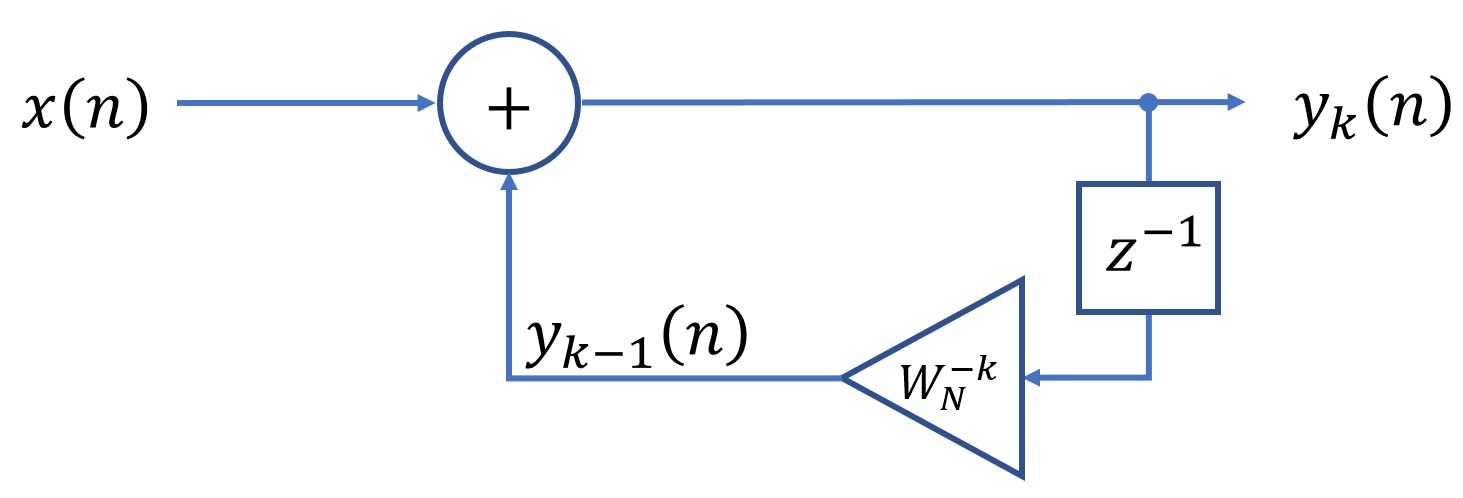
\includegraphics[width=\textwidth]{img/goertzel-1st.png}
  \captionof{figure}{格兹尔一阶滤波器系统示意图}
\end{figure}

对应的差分方程如下:
\begin{equation}
  y_{k}(n)=\omega_{N}^{-k}\ y_{k}(n-1)+x(n),\qquad \ y(-1)=0
\end{equation}

依照此差分方程进行迭代运算,迭代到$n=N$时即可通过\Cref{eqn:output}得到$X(k)$.
\medskip

格兹尔算法与离散傅里叶变换的相似处在于他们都可以分析某个特定频段的离散信号,
不同处在于,格兹尔算法每次迭代都使用实数乘法,不需要涉及到复乘运算。
虽然在全频域的计算上,格兹尔算法的复杂度高于其他的傅里叶变换算法,
但是它能区段式的分析每个小区段的频率组成,因此可以编写成较简单的运算架构,
在实际处理器的数值计算中更有效率。

\subsubsection{格兹尔算法---C语言实现}
由于我们只关注信号在一个频点上是否显著,因此可使用格兹尔算法的能量谱形式:

\begin{minted}{c}
double goertzel_power(int num, int freq, const double *data)
{
  double omega, cosine, coeff, q0, q1, q2;

  int k = (int) (0.5 + ((num * freq) / (double)SAMPLING_RATE));
  omega = (2.0 * M_PI * k) / num;
  cosine = cos(omega);
  coeff = 2.0 * cosine;
  q1 = 0;
  q2 = 0;
  for (int i = 0; i < num; i++)
  {
    q0 = coeff * q1 - q2 + data[i]*hanning_1024[i];
    q2 = q1;
    q1 = q0;
  }
  return q1*q1 + q2*q2 - coeff*q1*q2;
}
\end{minted}

其中,变量\cinl{q0,q1,q2}分别代表IIR滤波器的当前及前两次输出。

在STM32F103平台(主频\SI{72}{MHz},无硬件浮点单元)上实测,在输入长度为1024时,
算法总耗时\SI{4.1}{ms}左右。相对应的,一次1024点FFT(使用前述库函数)耗时\SI{5.4}{ms}。
考虑到我们一次解码4个点,相应地就需要运行4次格兹尔算法,因此相比FFT来说并没有优势。
